\documentclass{article}
\usepackage[letterpaper, margin = 1 in]{geometry}
\usepackage{graphicx}
\graphicspath{.}
\usepackage{float}

\begin{document}

\noindent \textbf{Thickness} \\ \\
Vortex of strength $\Gamma$ = -0.02 started upstream at (-4.5,0.04). Given that the airfoil in consideration is now a NACA 0012 and not a flat plate, it is expected that the frequency spectrum obtained will not match with Sears. As detailed in Lysack (2011), a thickness correction can be written for a given airfoil profile. For the thickness of the NACA 0012, the expression was adjusted accordingly and compared to the results obtained from the BEM simulation. The resulting expressing is detailed below. 

\begin{equation}
H(f)^2 = (\pi \rho c v_o U_{\infty})^2\Bigg(1 + \epsilon + \frac{\delta_{TE}}{2\pi} \Bigg )^2 S(f)^2 exp\Bigg[-\beta(\tau)\frac{fc}{U_{\infty}}\Bigg]
\end{equation}

\noindent where S(f) is the Sears function and $\beta(\tau)$ is a curve fit parameter which controls the rate of high frequency attenuation. This varies for the airfoil being used. The fitting parameter used was developed by Moriarty et al. (2005). Their formula leads to an attenuation coefficient of: 
\begin{equation}
\beta(\tau) = \frac{2\pi ln(10)}{10} \big[1.123D(\tau) + 5.317D(\tau)^2 \big]
\end{equation}
where $D(\tau) = (\tau/c)_{1\%} + (\tau/c)_{10\%}$ is based on the thickness to chord ratio at 1$\%$ and 10$\%$ chord. 

\begin{figure}[h]
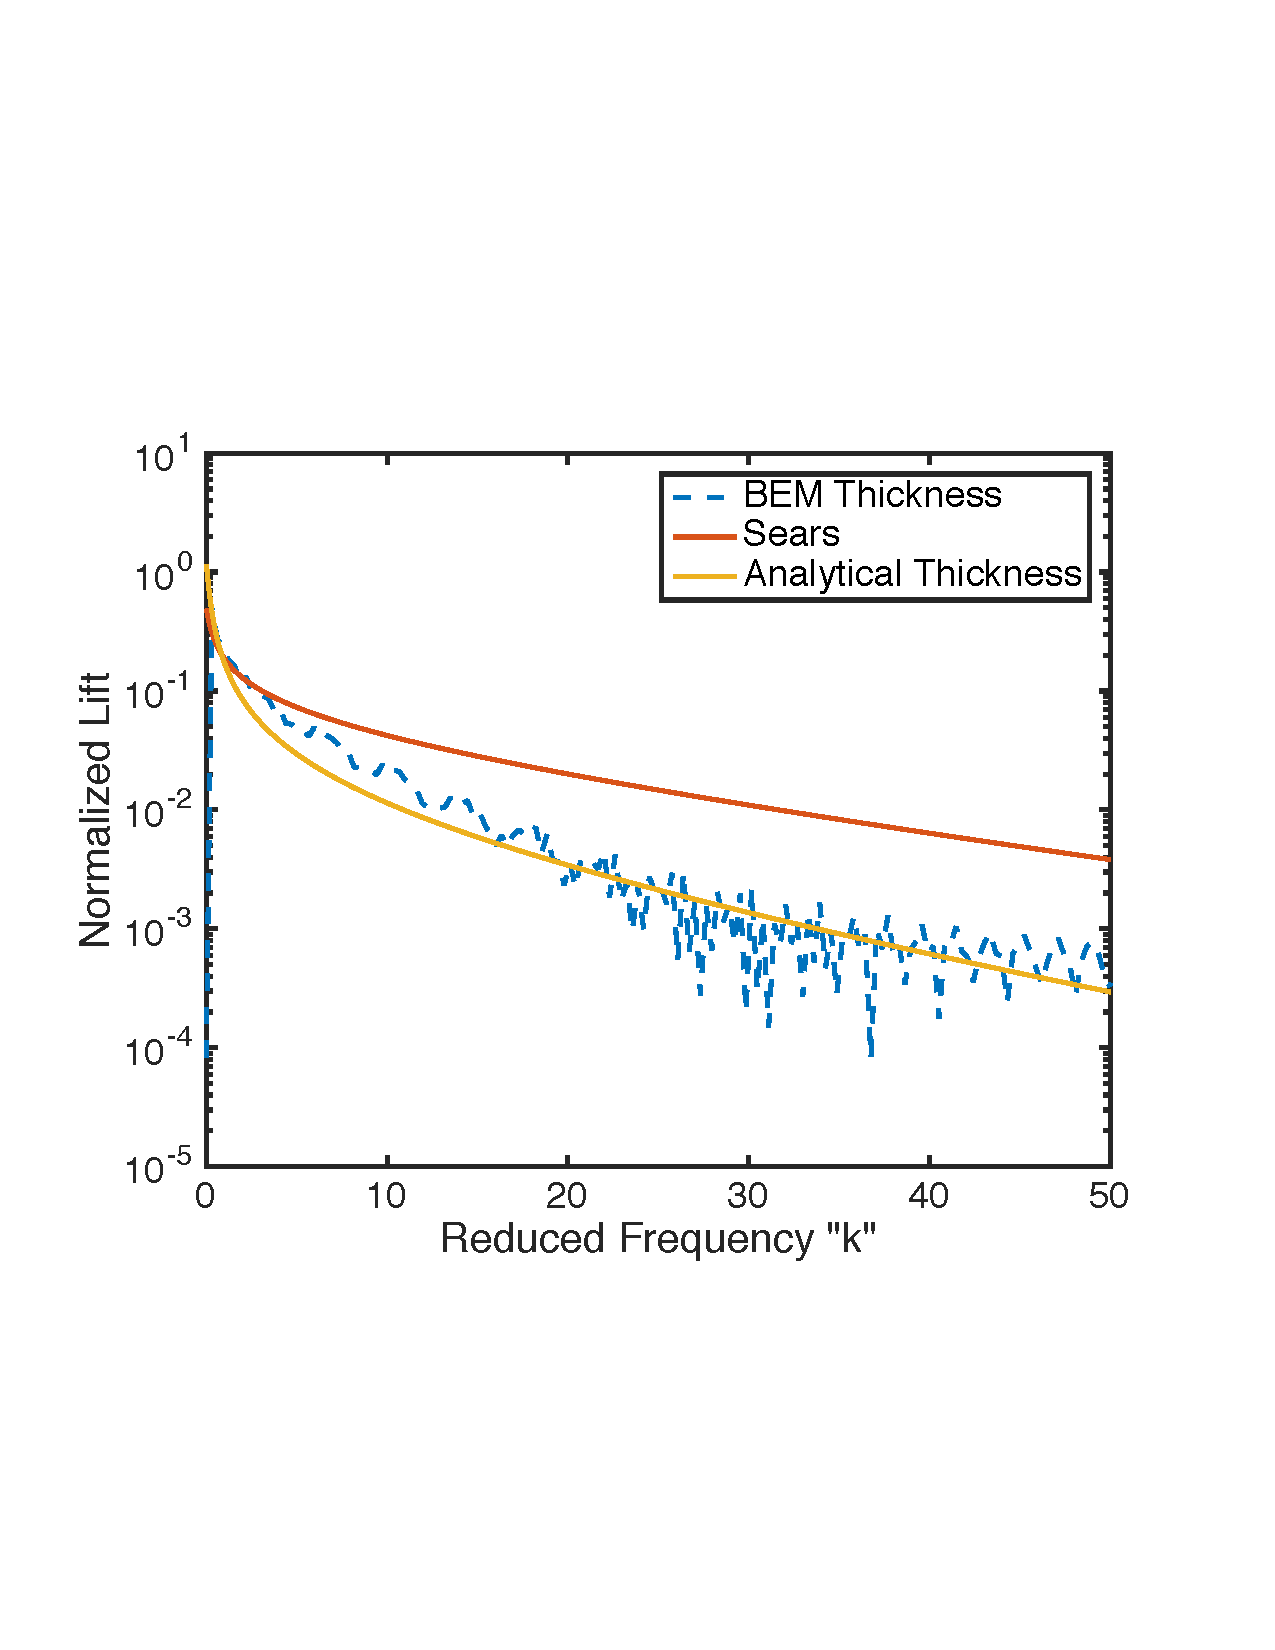
\includegraphics[width = 4 in, height = 3 in]{BEM_Compare}
\centering
\caption{Comparison of Lift Spectrums}
\end{figure}

\newpage

\noindent When defining the geometry for the BEM code, one can either select the airfoil to be discretized using a linear or a cosine spacing. It was interest to see what effect a different discretization would have on the results of the transform. Shown in the figure below is the lift spectrum results for a NACA 0012 airfoil discretized using a cosine spacing. The previous results shown in figure 1 was discretized using the linear spacing approach. 

\begin{figure}[h]
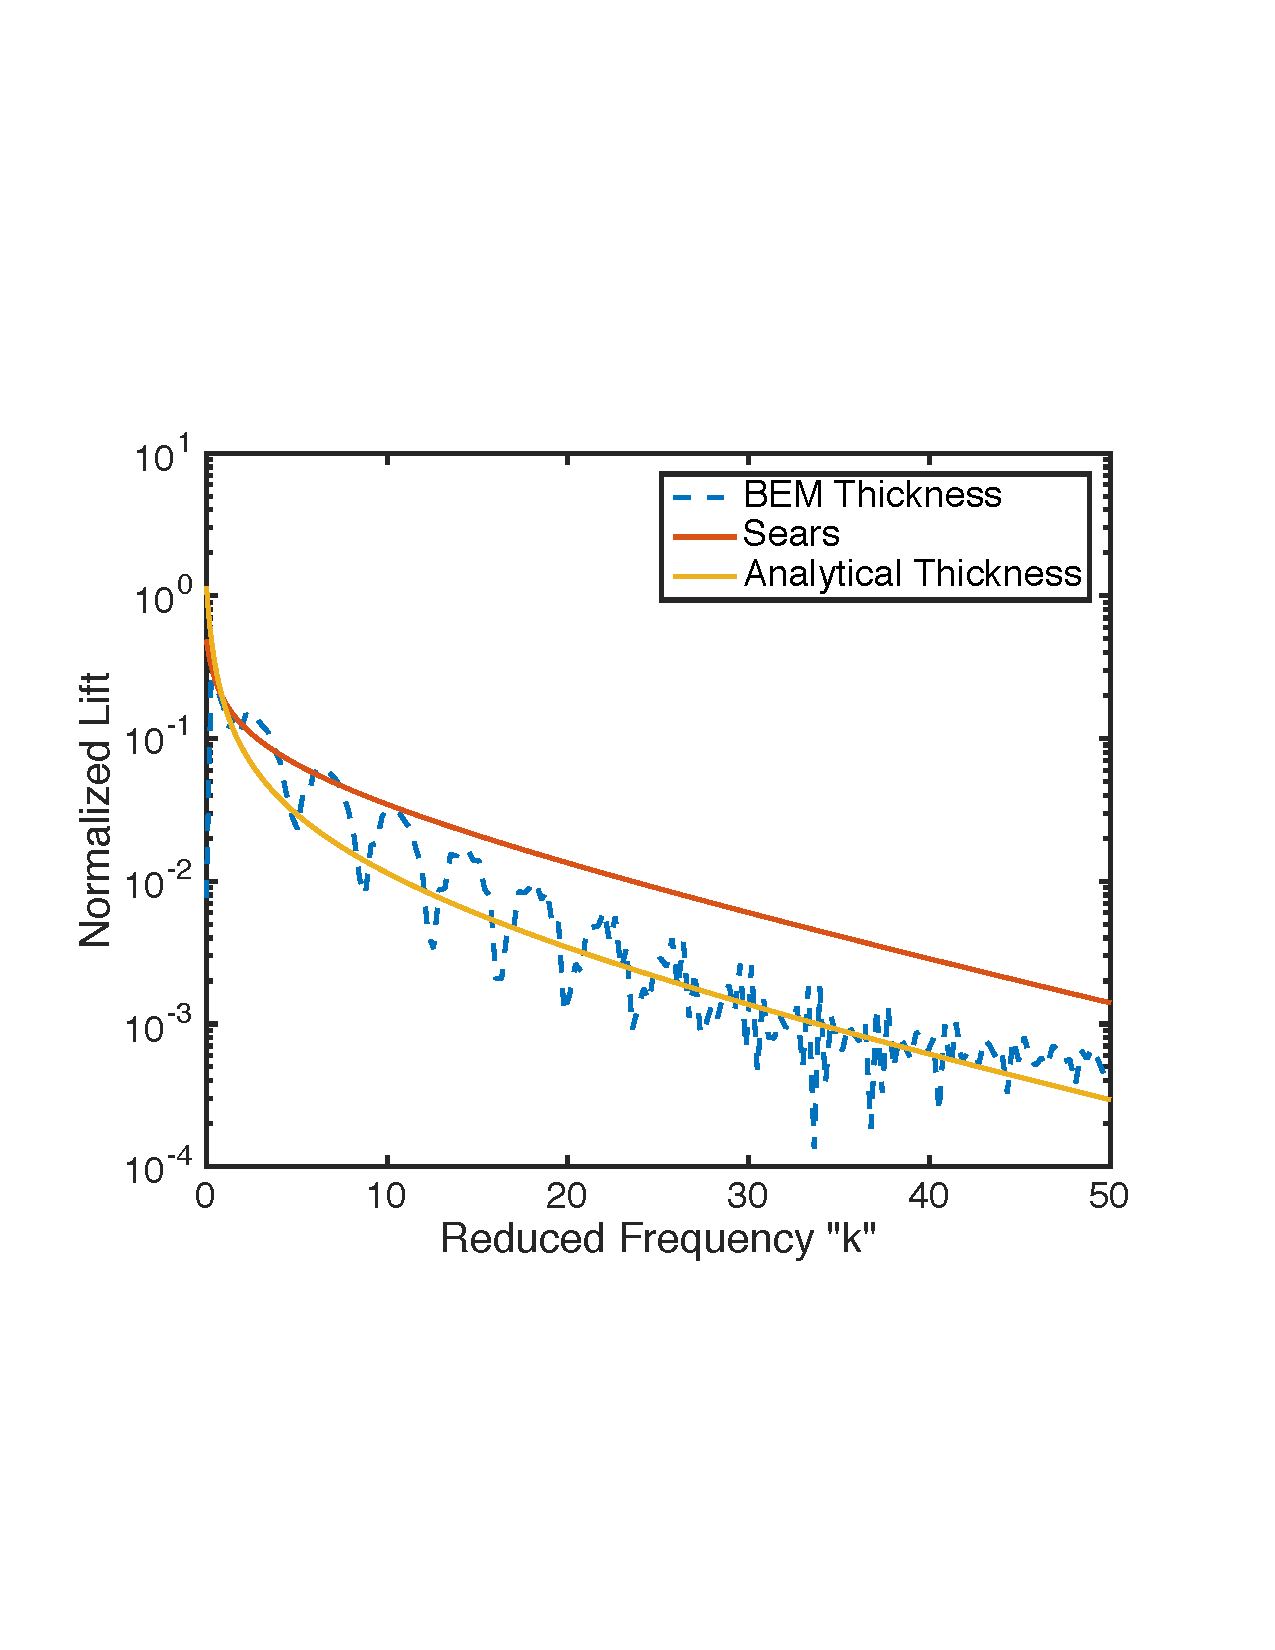
\includegraphics[width = 4in, height = 3.2in]{BEM_Cosine_0012}
\centering
\caption{Lift Spectrum for NACA 0012 - cosine spacing}
\end{figure}


\end{document}


